
\section{Introduction}

This chapter and the next review the epistemology of knowledge and the role of motivation, trust, and power relevant to tacit knowledge sharing. Each chapter presents a number of broad propositions that inform our exploratory mixed-method analysis of tacit knowledge sharing in open innovation. \medskip

The previous chapter conceptualised an open innovation partnership as a temporary knowledge network deliberately set up to achieve a specific innovation outcome within a market-relevant time frame. It also highlighted the importance of tacit knowledge for open innovation. Tacit knowledge exchange is a socially intensive process, and embracing a network perspective offers valuable insights into the self-organising (endogenous) and external (exogenous) factors influencing tacit knowledge transfer processes. This chapter considers the nature of knowledge and how this affects absorptive capacity and knowledge brokerage in open innovation. As a reminder, absorptive capacity is the ability of a firm to value, acquire, assimilate, transform, and exploit new external knowledge \citep{cohen1990absorptive}. Knowledge brokerage is about connecting people with knowledge to those who need it. \medskip

Although there are many aspects to managing knowledge flows across organisational boundaries, this chapter makes the case that open innovation is mainly about facilitating the interaction between know-how (practical knowledge on how to accomplish something) and know-what (factual knowledge) \citep{winter1987knowledge,garud1997distinction}. Other forms of knowledge are know-who (knowing who has relevant know-how), know-why (scientific understanding), and know-when (knowing when to apply know-how) \citep{hulme2014editorial}. We use theoretical concepts to formulate propositions about tacit knowledge sharing in open innovation. This study is exploratory, and the propositions are less about testing specific hypotheses about tacit knowledge sharing as they are about gaining a deeper and more nuanced understanding of the social mechanisms that underpin tacit knowledge sharing. 

\section{The nature of knowledge}

Traditionally knowledge is considered a justified true belief \citep{bolisani2018elusive}. For those who embrace a positivist worldview, truthfulness is the main feature of knowledge. Positivists see knowledge as objective, static, and absolute. Others who embrace a constructivist or pragmatic worldview place more weight on justified beliefs. For them, the utility of knowledge is more important than truthfulness \citep{bolisani2018elusive}. \citet{spender1996organizational} observes that \enquote{knowledge is less about truth and reason and more about the practice of intervening knowledgeably and purposefully in the world}. What matters is not what we know, but knowing how to apply our knowledge \citep{ryle1949concept,orlikowski2002knowing}. \medskip

It is helpful to think about how people know things. Two perspectives dominate the theory of knowledge: rationalism and empiricism. Rationalism argues that knowledge is the result of a reasoning process. Knowledge exists in our minds. What is observed or sensed does not constitute knowledge \citep{russell2009human}. On the other hand, empiricism argues that knowledge is a product of our sensory interface with the real world \citep{bolisani2018elusive}. The distinction between rationalism and empiricism becomes useful when interpreted to mean that humans know in two ways, either through experience or reasoning. When these two ways of knowing interact, new knowledge is created \citep{spender1996making,bolisani2018elusive}. \citet{cook1999bridging} consider knowledge in terms of the epistemology of possession and the epistemology of practice. The epistemology of possession treats knowledge as something people possess (know-what or know-that), whereas the epistemology of practice refers to knowing how to enact knowledge in practice (know-how). Know-how is the ability to put know-what into practice \citep{cook1999bridging,tsoukas2001organizational, marabelli2014knowing}. \medskip

\citet{polanyi1966tacit} states that people often know how to do things by adhering to a set of rules they are unaware of. He refers to this unknown set of rules for skilful action as tacit knowledge (or tacit knowing, to be more precise). People accumulate tacit knowledge through observation, imitation, and repeated interaction. Tacit knowledge is deeply rooted in personal experience \citep{nonaka1995knowledge}. Not only is tacit knowledge embodied in the minds and actions of individuals, but it is also manifest in group practice and culture, usually in the form of unwritten rules and procedures \citep{munoz2015tacit}. \medskip

Innovation is about transforming ideas into reality, a process that involves applying know-how to new or existing knowledge in novel ways \citep{van1986central,quintane2011innovation,garud2013perspectives}. This perspective implies that open innovation is less about managing knowledge flows as it is about bringing know-how and know-what together. Sharing know-how enables others to learn the practice that entails the know-how. Thus, open innovation entails helping others develop the ability to apply knowing and knowledge in new and different contexts \citep{van1986central,goksel2016can}. 

\section{Knowledge networks}

A knowledge network connects individual and organisational actors across organisational, spatial, and disciplinary boundaries to create, share, or apply a body of knowledge \citep{pugh2013designing}. Some researchers distinguish between a knowledge network and a social network \citep[e.g.][]{yayavaram2008decomposability,wang2014knowledge,brennecke2017firm}. Such a distinction is warranted if one treats people and knowledge as separable entities. As tacit knowledge is embodied in the minds and actions of people, such a distinction is not appropriate for this thesis. Instead, this thesis treats a knowledge network as a social network, where ties represent social interactions between knowledgeable actors. \medskip

The value a firm can extract from its knowledge network depends on the reach of the firm's ties to diverse and distant partners, the richness of knowledge embedded in the network, and how easily a firm can harness its network resources \citep{gulati2011networks}. We can describe a firm's reach in terms of its weak knowledge ties \citep{hansen1999search}. Actors connected by strong ties often share similar interests and are privy to the same knowledge. Strong ties tend to make people look inward and be less receptive to external knowledge. Actors connected by weak ties tend to mix in different social circles and are thus more exposed to different knowledge and opportunities \citep{granovetter1973strength}. \medskip

Regarding the richness of knowledge resources, the depth of knowledge and quality of knowledge is of primary importance, as this determines the potential value of the knowledge resource \citep{davenport1998working,kane2005knowledge}. The depth of knowledge reflects its usefulness for problem-solving. Addressing simple problems requires basic know-how. As problems become increasingly complex, higher levels of cognition are required. More profound know-how is required to solve more challenging problems \citep{webb2002depth,bennet2008depth}. We can describe the quality of knowledge in terms of its usability, completeness, currency, and accuracy \citep{wixom2005theoretical}. \medskip

How easily open innovation partners can harness knowledge embedded in a network depends on several factors. Complex knowledge usually has a significant tacit component to it. Transferring complex knowledge is difficult because it involves transferring know-how between partners as well. The human dimension of such knowledge makes it particularly \enquote{sticky} \citep{von1994sticky,szulanski2003sticky}. \medskip

Different levels of openness can lead to a breakdown of trust and loss of enthusiasm between open innovation partners \citep{laursen2014paradox,dragsdahl2019perspective}. How open a firm is in an open innovation partnership is usually determined by its appropriability regime. An appropriability regime refers to the mechanisms put in place by a firm to prevent knowledge from being appropriated by imitators \citep{teece1998capturing,hurmelinna2008appropriability}. It is not always clear to other firms in the partnership how this works. One way to resolve this is by making appropriability regimes more explicit from the outset \citep{gama2019managing}. \medskip

Relative differences in absorptive capacity between open innovation partners can also impede efforts to combine or integrate different ways of knowing \citep{vanhaverbeke2007connecting,lichtenthaler2016absorptive}. Spatial proximity is another factor. Achieving interaction between different ways of knowing is difficult when partners are not close to each other \citep{wineman2009spatial,roper2018knowledge}. \medskip

When examining the structure of a knowledge network, a structural hole refers to gaps between separate groups of people \citep{burt2000network}. Groups on either side of the structural hole are privy to different knowledge. Members of tightly-knit groups are more likely to work with tacit knowledge in the form of mutually understood, unwritten language and routines to coordinate with one another \citep{burt2007secondhand}. Structural holes present an opportunity to broker knowledge exchanges between otherwise disconnected groups of people. A knowledge network with an abundance of structural holes facilitates innovation by allowing strategically placed actors to access and combine diverse knowledge in novel ways \citep{burt2004structural,sparrowe2011publishing}. \medskip

Because tacit knowledge familiar within groups is likely to be invisible to other groups, it can yield a premium to brokers who can coordinate such knowledge across the groups \citep{burt2007secondhand}. While brokerage across structural holes in a disconnected knowledge network is the source of value, network closure is critical to realising the value buried in structural holes \citep{burt2004structural,rost2011strength}. Network closure refers to a human tendency to form into social groups. More closed networks with fewer structural holes promote trust and reduce opportunism leading to more productive collaboration from knowledge sharing \citep{ahuja2000collaboration}. \medskip

In summary, we conceive an open innovation partnership as a temporary knowledge network set up to achieve a specific innovation outcome. Extracting value from a knowledge network depends on network reach, the depth and quality of relevant knowledge embedded in the network, and the ability of partners to leverage knowledge resources. While connections across structural holes are a source of value in a knowledge network, network closure is vital for realising the value buried in structural holes. Hence, \bigskip

\begin{tcolorbox}
\textit{\textbf{Proposition 1a:} Open  innovation  requires  practitioners  to  connect across organisational and disciplinary boundaries so that they can apply their know-how in novel ways. (Sub-research Question 1).}
\end{tcolorbox}

\section{Absorptive capacity} 

Thus far, we have examined how to capture value from temporary knowledge networks by bridging structural holes and achieving network closure. We need to promote interaction between those open innovation partners who possess the knowledge and other partners who know how to apply it. The ability to generate value through such interaction is contingent on the absorptive capacity of the latter \citep{vanhaverbeke2007connecting,lichtenthaler2009capability,robertson2012managing,xia2016unpacking}. \medskip

Absorptive capacity is the \enquote{ability of a firm to recognise the value of new, external information, assimilate it, and apply it to commercial ends} \citep{cohen1990absorptive}. Despite being the subject of countless studies, the extent to which absorptive capacity contributes to firm performance is still an open issue \citep{omidvar2013revisiting,duchek2013capturing}. Open innovation puts the organisational practices used to source external knowledge into sharp focus. Treating an open innovation partnership as a temporary knowledge network opens new avenues to explore practices that build absorptive capacity \citep{vanhaverbeke2007connecting,xia2016unpacking}. \medskip

What is absorptive capacity exactly? \citet{cohen1990absorptive} embrace a cognitive approach to absorptive capacity by connecting ideas from individual learning to organisations. According to them, the amount of experiential knowledge a firm can accumulate through its employees determines its absorptive capacity. They view the relationship between absorptive capacity and the level of experiential knowledge as a positive feedback loop, where an increase in absorptive capacity improves the level of relevant knowledge, which in turn further increases absorptive capacity. Mediating this feedback loop is the environment the firm operates in \citep{van1999coevolution}. \citet{lane1998relative} suggest that absorptive capacity is more about the ability of a firm to learn from another. This ability is a function of the extent to which firms have overlapping knowledge bases and the extent to which they socially interact \citep{dyer1998relational,nooteboom2000learning}. \medskip

Early studies paid little attention to the processes that build absorptive capacity leading \citet{zahra2002absorptive} to re-conceptualise absorptive capacity as a dynamic capability that integrates internal processes for acquiring, assimilating, transforming, and exploiting external knowledge. They describe knowledge acquisition as the ability of a firm to identify and acquire externally generated knowledge critical to its operation. Knowledge assimilation encompasses the processes used by a firm to make sense of externally sourced knowledge, whereas knowledge transformation refers to the processes used by a firm to integrate assimilated external knowledge with existing internal knowledge. Knowledge exploitation is about the processes used by a firm to enhance existing competencies or create new ones by incorporating acquired and transformed knowledge into its operations. \citet{zahra2002absorptive} distinguish between potential absorptive capacity, namely the capability to acquire and assimilate new external knowledge, and realised absorptive capacity, which is the capability to transform and exploit knowledge. They suggest that the ratio of realised absorptive capacity to potential absorptive capacity measures the efficiency of an organisation at leveraging absorbed knowledge. \citet{zahra2002absorptive} also highlight the importance of social mechanisms that connect people who acquire external knowledge with people inside the firm who can apply this knowledge. \citet{jansen2005managing} find coordination capabilities, namely brokerage, shared decision-making and job rotation, enhance potential absorptive capacity, whereas socialisation capabilities increase realised absorptive capacity. \medskip

\citet{todorova2007absorptive} highlight how different appropriability mechanisms and power relations may influence absorptive capacity.  Firms may employ several mechanisms to protect their knowledge from being appropriated by others. How and when these are applied is often unclear and can create tension between knowledge sharing and knowledge protection practices \citep{gama2019managing}. Firms do not want to leak valuable knowledge as quickly as they absorb it \citep{todorova2007absorptive}. The tension between knowledge sharing and knowledge protection can thwart inter-organisational learning needed to overcome relative differences in absorptive capacity \citep{dragsdahl2019perspective,gama2019managing}. Regarding power relations, \citet{todorova2007absorptive} claim power relations inside the firm moderate the assimilation and transformation of knowledge, while power relations between partners moderate the relationship between absorptive capacity and competitive advantage.  \citet{easterby2008absorptive} observe that political acts by brokers affect access to external knowledge, while diffusion of knowledge within a firm depends on the extent to which employees are empowered. \citet{easterby2008absorptive} also highlight the importance of boundaries and how these affect absorptive capacity processes. The permeability of boundaries determines the ease of transferring knowledge. They consider power and boundaries as central features of a process view of absorptive capacity. \medskip

\citet{marabelli2014knowing} interpret a firm's absorptive capacity in terms of the epistemology of possession and the epistemology of practice. They differentiate between knowledge that resides in people's minds, easily spread by individuals who can develop a shared understanding with others and sticky knowledge enacted in practice. The epistemology of practice treats absorptive capacity as a capability that emerges when applying knowledge in practice. \citet{marabelli2014knowing} argue that a practice-based perspective provides a more nuanced perspective of power and how it shapes absorptive capacity. They refer to prohibitive and productive power (also referred to as power-over and power-to, respectively). Prohibitive power focuses on the power of organisational actors to control knowledge and achieve objectives at the expense of others. On the other hand, productive power focuses on empowering (or dis-empowering) actors to change knowledge practices. \medskip

\citet {lichtenthaler2016absorptive} argues that past studies have overlooked the negative consequences of building absorptive capacity. These include challenges in capturing value from knowledge, overemphasising prior-related knowledge, and inter-dependencies between internal processes. The challenges around capturing value relate to the capabilities needed to manage increasingly sophisticated knowledge and the rising cost of capability development. \citet{lichtenthaler2016absorptive} claims that firms struggle to capture value from tacit knowledge, and prior-related knowledge may be of limited use when it comes to adapting and transforming knowledge for use in new contexts. Firms may not benefit from externally sourced knowledge because it may decay over time. \medskip

 How partners manage their appropriability regimes may stand in the way of this. Absorptive capacity is also affected by the way power is exercised at both the individual and organisational level \citep{todorova2007absorptive}. \bigskip

\begin{tcolorbox}
\textit{\textbf{Proposition 1b:} Reducing cognitive distance between open innovation partners  requires  significant  social  interaction  to support learning and the application of knowledge in practice (Research Question 1).}
\end{tcolorbox}

\section{Knowledge brokerage}

Brokerage may be defined as the \enquote{behaviour by which an actor influences, manages, or facilitates interactions between other actors} \citep{obstfeld2014brokerage}. Knowledge brokers make connections between those who need knowledge and those who have it, i.e. they apply their know-who to connect people with the relevant know-how \citep{davenport1998working}. From a network perspective, brokers bridge structural holes. They can use their position to influence access to knowledge resources through their network of weak ties \citep{burt1992structural,hanneman2005introduction,davis2010agency,simpson2011network,stovel2012brokerage}. From a practice perspective, brokers facilitate the integration and synthesis of knowledge provided by others. Both approaches invoke power, but a critical distinction between them is that brokers in open innovation partnerships are less likely to operate only out of self-interest \citep{lingo2010nexus,marabelli2016strategic}. \medskip

\citet{obstfeld2014brokerage} describe three strategic orientations to brokerage: \enquote{conduit}, \enquote{tertius gaudens}, and \enquote{tertius inungens} brokerage. Conduit brokerage is about a third party who transfers information, knowledge, or resources between two disconnected parties. The broker mediates rather than moderates the relationship between two others and may help them synthesise new knowledge. Tertius gaudens refers to \enquote{the third who enjoys} \citep{simmel1950sociology}. With tertius gaudens brokerage, the broker aims to exploit differences between two parties by either keeping them apart or playing one against another. In contrast, tertius iungens (\enquote{the third who joins}) brokerage is about a third-party who introduces two otherwise disconnected parties to each other and encourages them to collaborate (Table \ref{tab:brokerage}). \medskip

\begin{sidewaystable}
\resizebox{0.9\textwidth}{!}{
\begin{threeparttable}
\footnotesize
\setlength{\tabcolsep}{6pt}
\renewcommand{\arraystretch}{1}
\caption[Strategic brokerage orientations]{Strategic brokerage orientations \citep{obstfeld2014brokerage}.}
\label{tab:brokerage}
\begin{tabular*}{\textwidth}{>{\raggedright}p{5cm}>{\raggedright\arraybackslash}p{6cm}>{\raggedright\arraybackslash}p{6cm}>{\raggedright\arraybackslash}p{6cm}}
\toprule
& \multicolumn{1}{c}{Conduit} & \multicolumn{1}{c}{Tertius Gaudens} & \multicolumn{1}{c}{Tertius Iungens} \\ 
\midrule
& \begin{minipage}{0.2\textwidth} \centering 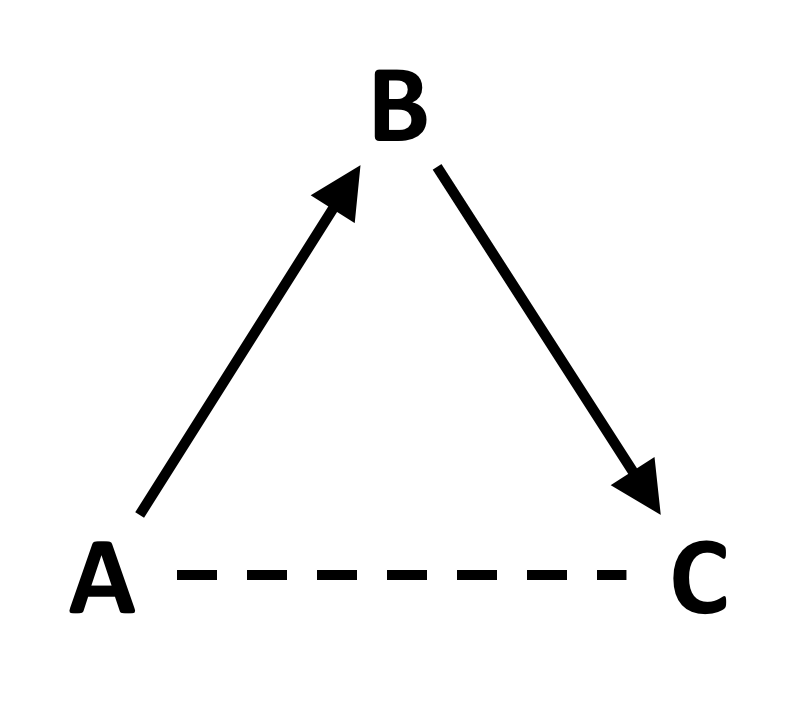
\includegraphics[width=0.7\linewidth]{Images/CDT_brokerage} \end{minipage}  & \begin{minipage}{0.2\textwidth} \centering 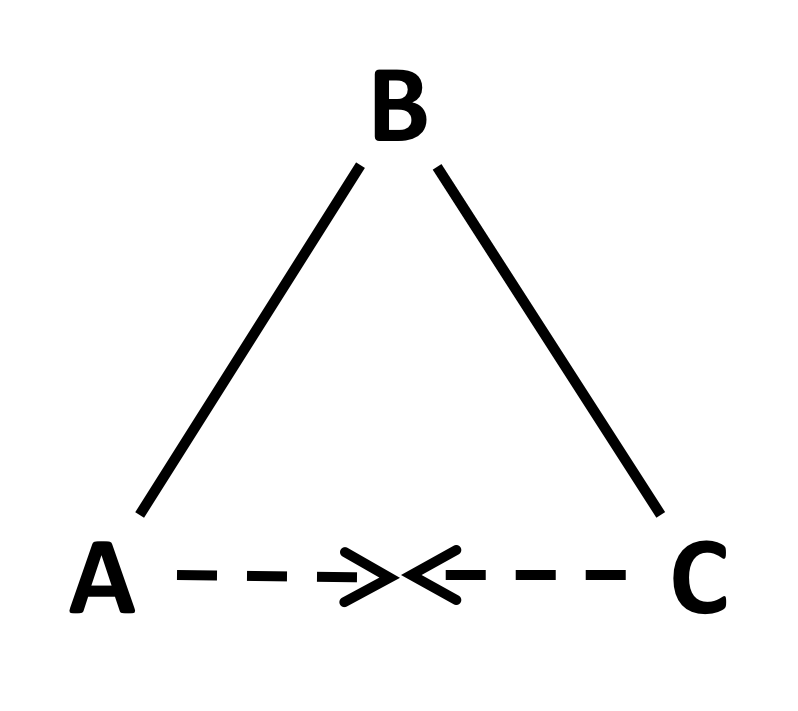
\includegraphics[width=0.7\linewidth]{Images/TG_brokerage_1} \end{minipage}  & \begin{minipage}{0.2\textwidth} \centering 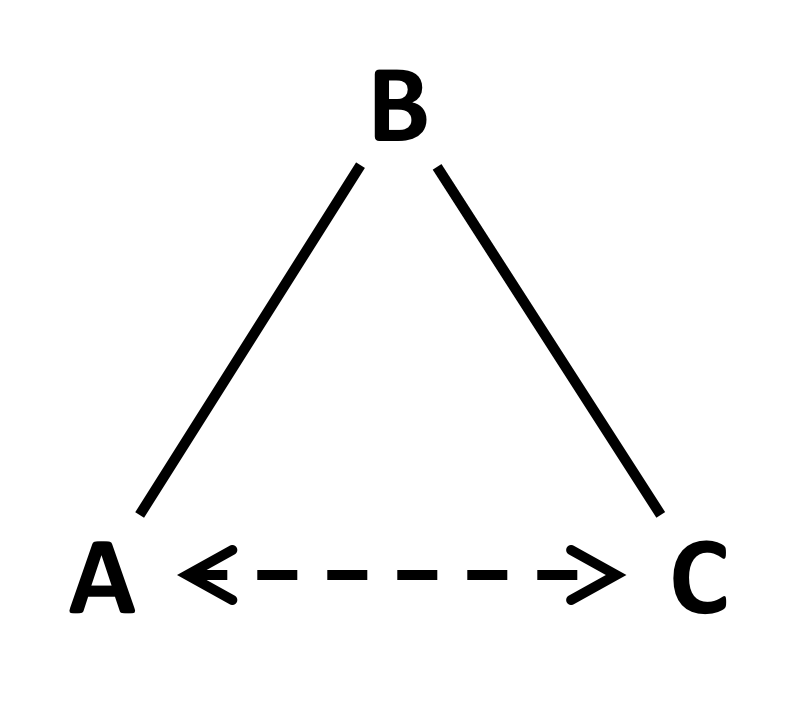
\includegraphics[width=0.7\linewidth]{Images/TI_brokerage} \end{minipage}   \\
&  & \begin{minipage}{0.2\textwidth} \centering 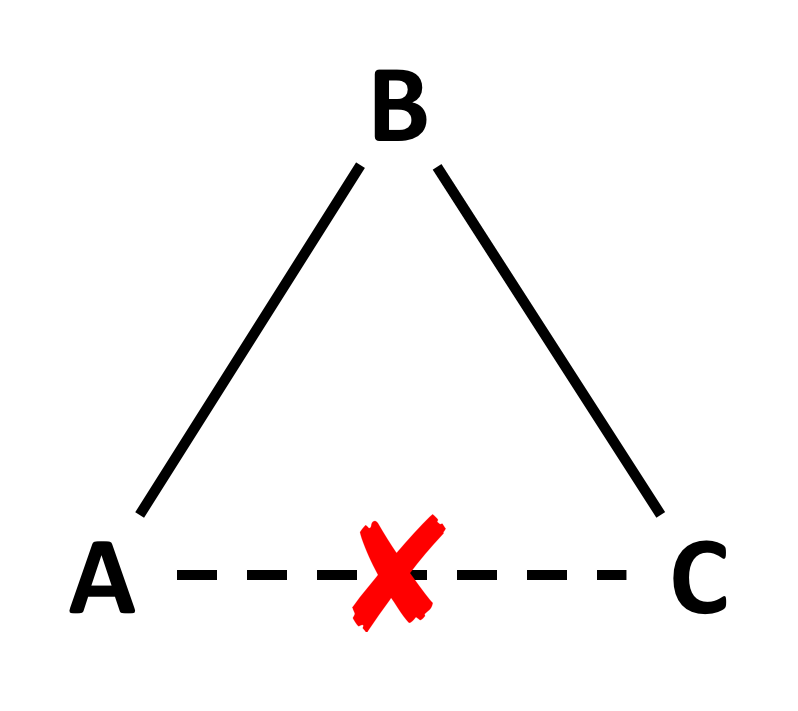
\includegraphics[width=0.7\linewidth]{Images/TG_brokerage_2} \end{minipage}  & \\
\midrule
Open network\\(absence of A-C tie) & B transfers information, knowledge, or other resources between A and C, where A and C have no prospect of meeting. & B plays A and C against one another or keeps A and C apart. & B introduces A and C where A and C have no prior tie. \\
\midrule
Closed Network\\(presence of A-C tie) & B facilitates transfer between A and C and may help synthesise new knowledge. & B cultivates conflict, competition, or separation between A and C (divide et impera) & B coordinates new collaborative action between A and C.  \\ 
\bottomrule
\end{tabular*}
\end{threeparttable}
}
\end{sidewaystable}

Each orientation expresses a different power dynamic. Whereas tertius gaudens brokerage is about exercising power over others, conduit and tertius iungens brokerage are mostly about empowering others \citep{fleming2007collaborative,obstfeld2014brokerage}. Skilled brokerage often involves the selective deployment of these approaches with different actors or for different objectives. Different combinations of tertius iungens and tertius gaudens behaviour are necessary to tailor brokerage strategies to match the situation \citep{lingo2010nexus,obstfeld2014brokerage,quintane2016brokers}. \medskip

Brokerage is also transient. The ability to engage in tertius gaudens brokerage diminishes when other actors engage in balancing operations to avoid or side-step power-dependencies \citep{emerson1962power}. Likewise, once a broker has introduced one actor to another through conduit or tertius iungens brokerage, their job of empowering others is complete \citep{obstfeld2014brokerage}. Brokers who have outlived their usefulness in a particular situation often seek out new brokerage opportunities. In that way, brokers drive the expansion and evolution of existing networks \citep{obstfeld2014brokerage,quintane2016brokers}. \medskip

From an open innovation perspective, tertius iungens brokerage is essential, especially in the early stages of collaboration, when many actors do not know fellow collaborators in partner organisations very well \citep{fleming2007collaborative}. Knowledge held by third parties is also likely to be unfamiliar, and brokers help others make sense of it. Once ties have formed through tertius iungens brokerage, conduit brokerage is needed to sustain trust and help synthesise and transform knowledge into novel ideas \citep{quintane2016brokers}. \medskip 

When actors belong to distinct groups, group membership allows one to categorise brokerage into five social roles. Brokers can operate as internal coordinators, as mediators, or in a liaison, representative, gatekeeper role depending on their network position \citep{gould1989structures}. Figure \ref{fig:gf_roles} depicts the network configuration of each role. The breakdown of broker roles should provide interesting insights into the character of the open innovation partnership \citep{spiro2013extended}. For example, a partner heavily invested in gatekeeping is likely to be more interested in empowering themselves at the expense of others in the partnership. Alternatively, partners who operate mostly in a representative or liaison broker role are likely to be more invested in the partnership and keen to empower others \citep{spiro2013extended}. \medskip

\begin{figure}
\centering
  \begin{subfigure}[b]{0.25\textwidth}
    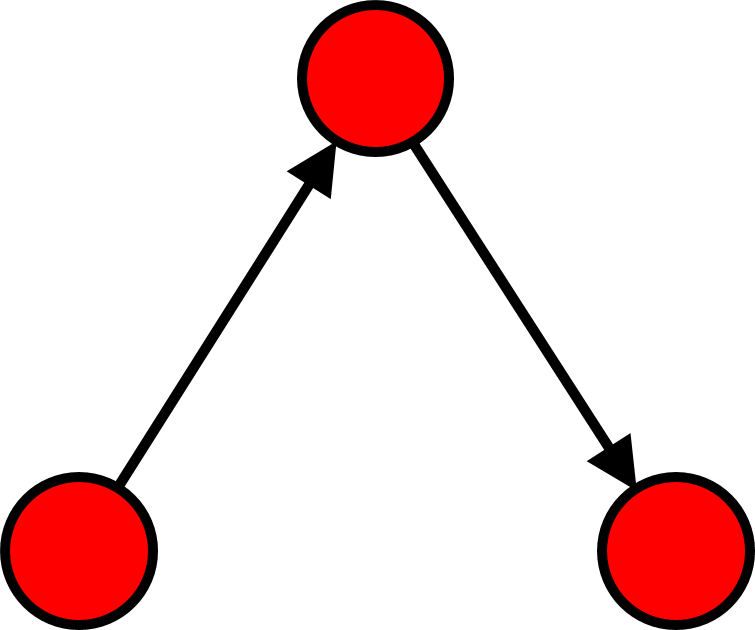
\includegraphics[width=\textwidth]{Images/w_I.png}
    \caption{Coordinator}
    \label{fig:1}
  \end{subfigure}
  \hspace{2em}
  \begin{subfigure}[b]{0.25\textwidth}
    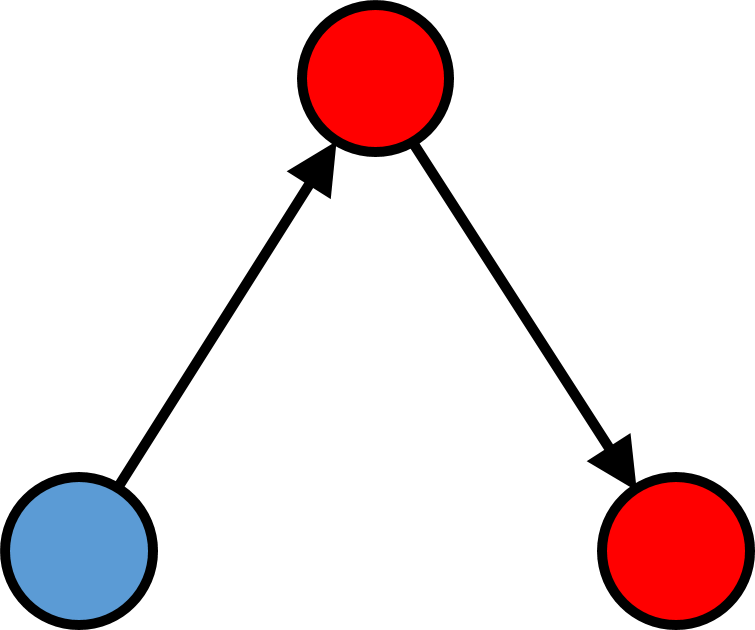
\includegraphics[width=\textwidth]{Images/b_OI.png}
    \caption{Gatekeeper}
    \label{fig:2}
  \end{subfigure}
  \hspace{2em}
  \begin{subfigure}[b]{0.25\textwidth}
    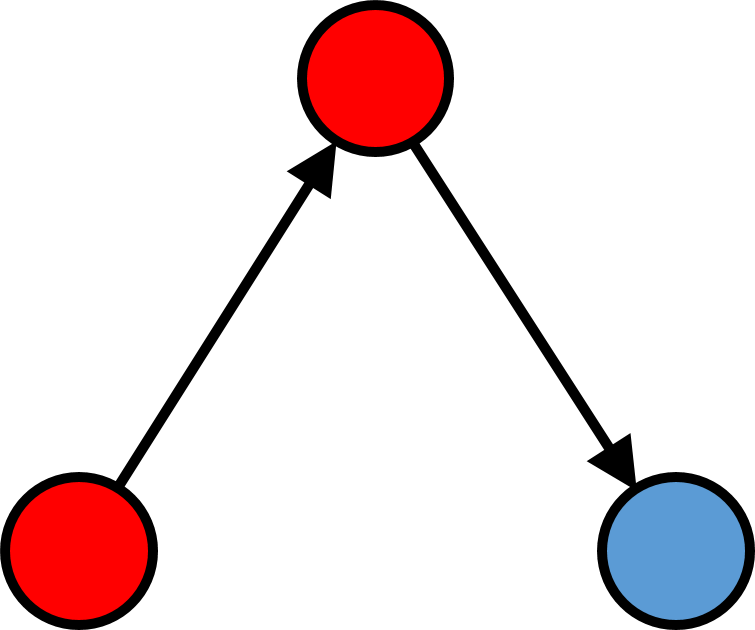
\includegraphics[width=\textwidth]{Images/b_IO.png}
    \caption{Representative}
    \label{fig:3}
  \end{subfigure}
  \par \bigskip
  \begin{subfigure}[b]{0.25\textwidth}
    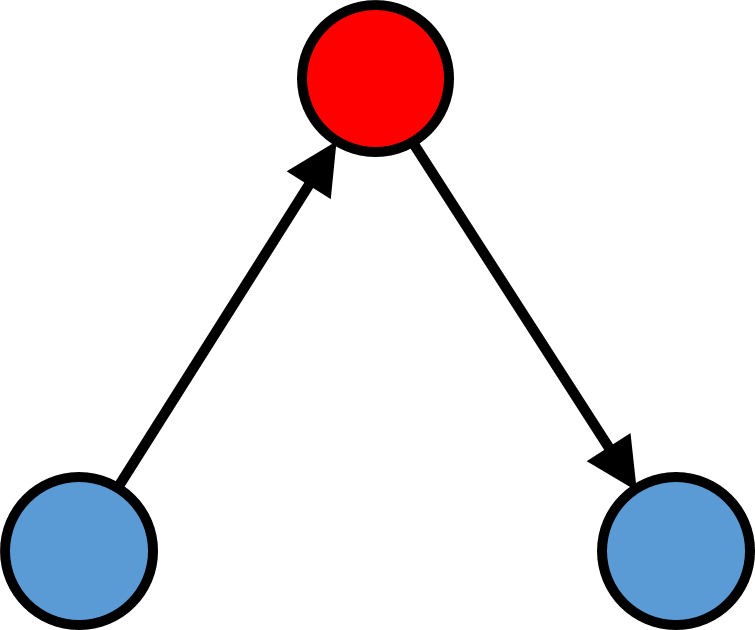
\includegraphics[width=\textwidth]{Images/w_O.png}
    \caption{Mediator}
    \label{fig:4}
  \end{subfigure}
  \hspace{2em}
  \begin{subfigure}[b]{0.25\textwidth}
    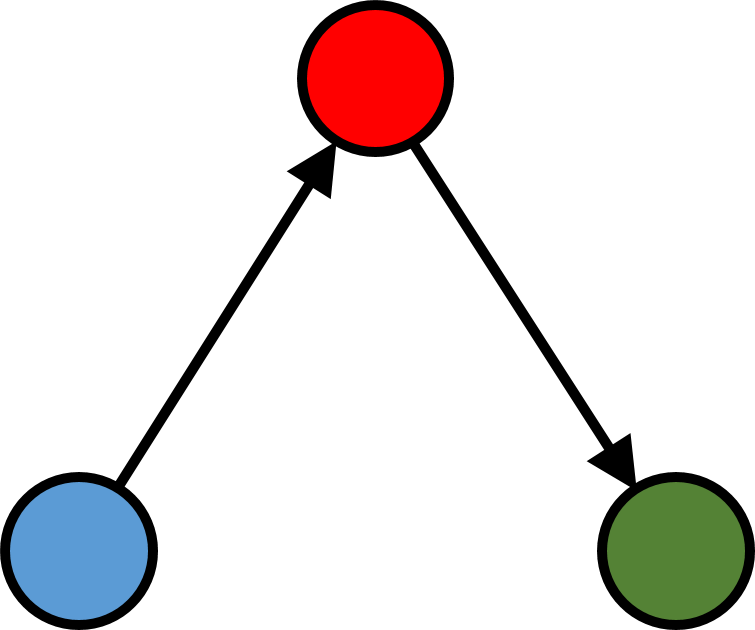
\includegraphics[width=\textwidth]{Images/b_O.png}
    \caption{Liaison}
    \label{fig:5}
  \end{subfigure}
  \caption[Broker roles]{\citet{gould1989structures} broker roles. The broker is the person receiving and sending ties. Colours represent different group affiliations.}%
    \label{fig:gf_roles}%
\end{figure}

Wrapping up, brokers play a vital role in establishing and growing knowledge networks. They are instrumental in identifying valuable sources of knowledge and connecting people who need knowledge with those who have it. Brokers also help others understand unfamiliar knowledge. From a structural perspective, brokers can use their position to their advantage (tertius gaudens brokerage). Brokers oversee collaborative efforts to integrate and synthesise knowledge to obtain both individual and mutual benefit (tertius inungens and conduit brokerage). Hence, \bigskip  

\begin{tcolorbox}
\textit{\textbf{Proposition 2a:} Successful open innovation requires a combination of skilled brokerage and network closure (Research Question 2).}
\end{tcolorbox}

\section{Summary}

Conceptualising an open innovation partnership as a temporary knowledge network allows one to use social network analysis to assess knowledge sharing practices in meaningful ways. Extracting value from the knowledge network depends on the absorptive capacity of partners. Whereas experiential knowledge is a vital component of absorptive capacity, applying knowing in practice also builds absorptive capacity. Applying knowing in practice requires good quality relationships. Brokers not only facilitate access to diverse sources of knowledge and expertise, but they also can help others make sense of unfamiliar knowledge. Brokers occupy powerful positions as they can control access to knowledge. However, they also can empower others by giving them access to knowledge. Patterns of brokerage can reveal much about power relations in open innovation partnerships. \medskip

Agency refers to the capacity possessed by people to act of their own volition within an existing social environment   \citep{bandura1989human,emirbayer1998agency}. As agency lies at the heart of tacit knowledge exchange, the next chapter explores how motivation, trust, and power affect agency in open innovation partnerships.